\chapter{Evaluation}
\label{sec:evaluation}

In this section, we explore a single
high-level question: is Sieve practical?
To answer this question, we integrated
Sieve with two applications. The first
was Open mHealth~\cite{omh}, an open-source
web service that allows users to analyze
their health data. We also integrated Sieve
with Piwigo~\cite{piwigo}, an open-source
online photo manager. We show that the
integration was straightforward, and that
the end-to-end application pipeline can
handle realistic workloads.

\begin{figure*}
\centering
  \subfloat[Encryption speed: ABE and Ed448 in randomized counter mode.]{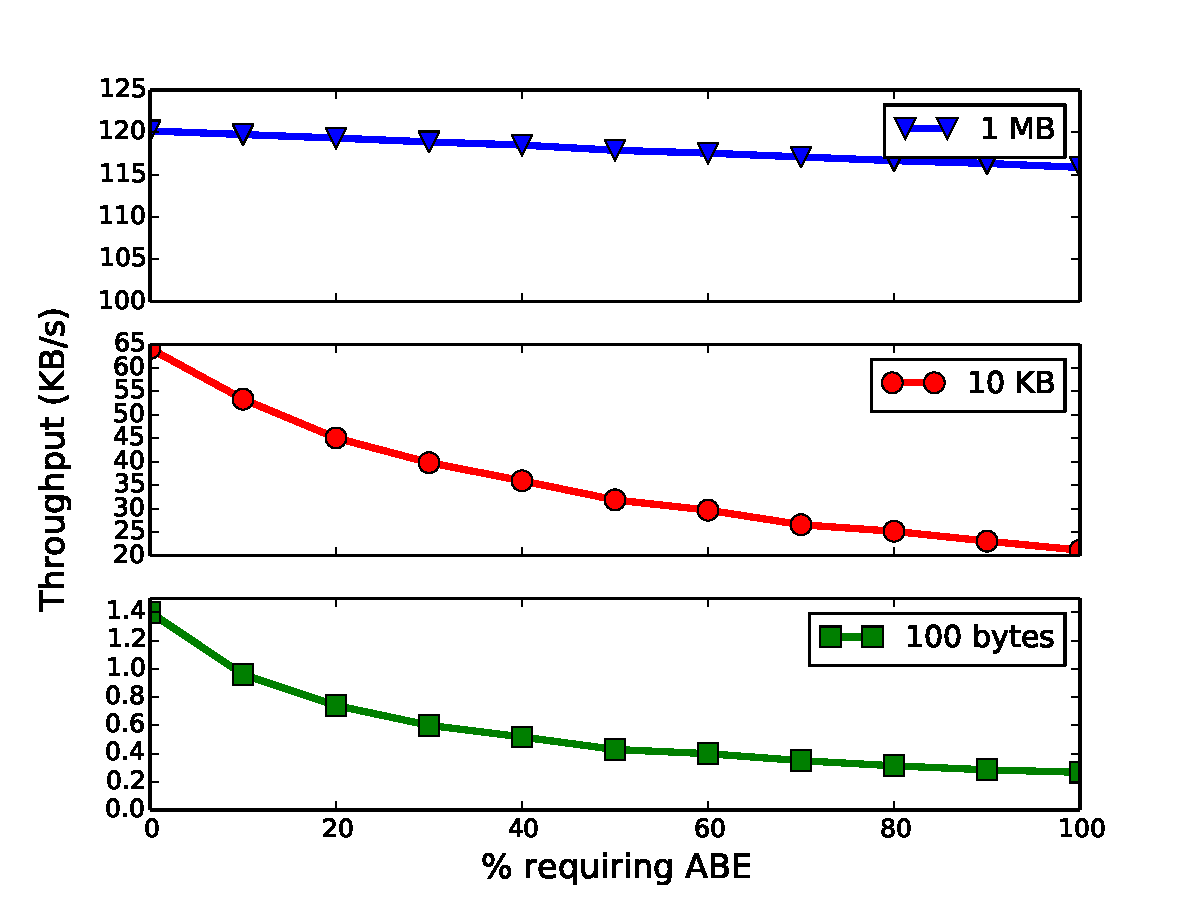
\includegraphics[width=0.48\textwidth]{figs/throughput1.pdf}\label{fig:throughput_ec}}
  \subfloat[Encryption speed: ABE and AES in CTR mode.]{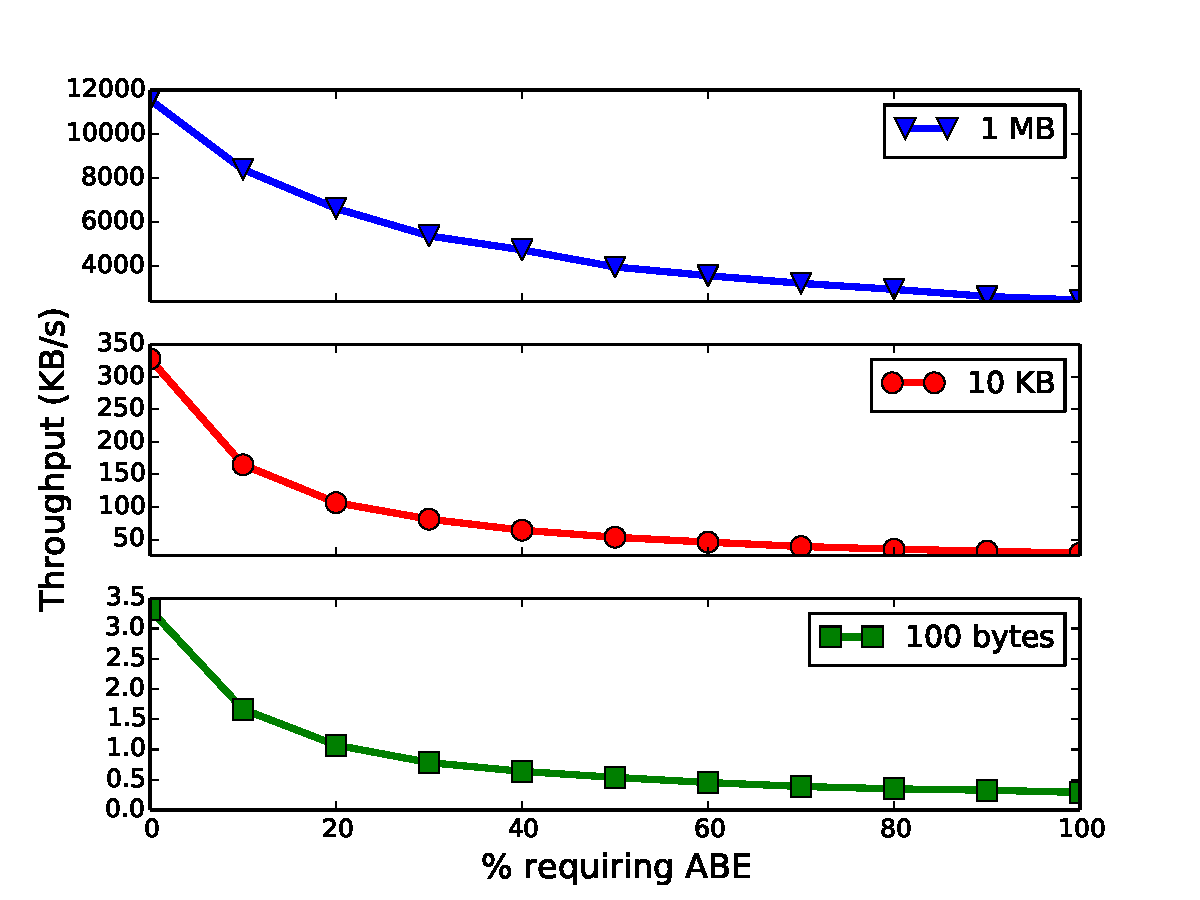
\includegraphics[width=0.48\textwidth]{figs/throughput2.pdf}\label{fig:throughput_aes}}
    \caption[ABE throughputs for Sieve]{Encryption throughputs for Sieve, as a function of 1) the size of
             the data to symmetrically encrypt, 2) the percentage of symmetric
             data encryptions which also require the ABE encryption of a
             metadata block, and 3) whether the cipher is AES or
             key homomorphic Ed448. All experiments assume that each metadata
             block has five attributes, and each ABE key has 10. Performance
             trends for decryption are similar.}
\label{fig:throughput}
\end{figure*}

All experiments ran on a machine with 2.4 GHz 10-core
Intel Xeon E7-8870 CPUs and 256 GB of RAM. We ran each
experiment 50 times, and we report the average
(standard deviations were small).
Sieve used 2048 bit RSA with SHA256 to sign
user objects. ABE operations used 224-bit MNT
curves~\cite{mnt224}. To symmetrically encrypt
those objects, Sieve used 128-bit AES in CTR
mode, or Ed448-Goldilocks elliptic curves in
randomized counter mode. The latter cipher is
key homomorphic, but the former is not; by
comparing Sieve's performance with these ciphers,
we could measure the cost of supporting key
revocation (\S\ref{sec:revocation}). All web
servers ran on the test machine's loopback
interface, to minimize network latency and
focus on Sieve's cryptographic overheads.

All GUIDs were 64 bits long. Thus, a metadata
block which contained a GUID and an AES key
was 24 bytes in size, whereas a metadata block
which contained a GUID and an Ed448 key was
64 bytes long.


\section{Case Studies}
\label{sec:integration}
We present the results of our integrations
with Open mHealth and Piwigo, and then discuss
these results.

\subsection{Open mHealth} 
Open mHealth allows
users to upload medical data to a web server
that will analyze the data and provide
explanatory visualizations. To integrate Sieve
with Open mHealth, we first modified the Open
mHealth client to upload data via the Sieve
client instead of directly to the Open mHealth
server. We then ran a Sieve import daemon on
the Open mHealth web server, configuring the
daemon with the data schema that the Open mHealth
analytics engine uses. These modifications
required approximately 200 lines of code
to be changed in the Open mHealth platform.

To test the end-to-end performance of the
application pipeline, we used Open mHealth's
data generator to create a week's worth of
health data. The data included information
like weight, blood pressure, physical activity,
and heart rate. Each day had approximately
14 data points. For each data point, the
Sieve client added attributes like the
date that the sample was collected, the
name of the associated user, and the type
of data represented by the sample. The Sieve
client used a single storage-based data 
structure to store the samples for an entire week.

The cost for the user to upload the first data point
at the beginning of a week was 0.56 seconds;
the cost was dominated by ABE encryption.
Uploading subsequent data points proceeded
at the throughput of the symmetric cipher,
requiring 17.1 ms per data point for AES,
and 38.5 ms for Ed448.

The mHealth server used the Sieve import daemon
to download user data. If the mHealth server
had no cached GUIDs or symmetric keys, then
importing a week of data required 1.1 seconds.
In this scenario, the server had to download
the metadata block, decrypt it with ABE,
download the raw data block, and then decrypt
that block using a symmetric cipher. If the
server possessed cached GUIDs and symmetric keys,
then importing a week of data took only 0.095
seconds with AES, and 0.75 seconds with Ed448.

\subsection{Piwigo} 
The standard Piwigo client
allows users to upload photos from local storage
to the Piwigo web service. We modified the client
to upload data to a Sieve storage provider, and
we modified the server-side Piwigo code to fetch
user data via the Sieve import daemon. These
modifications required approximately 250 lines
of new Piwigo code.

To test the end-to-end performance, we uploaded
a 375 KB photo which had three tags (location,
date, and username). If the Piwigo client used
AES as the symmetric cipher, the upload
required 0.57 seconds if a new, ABE-encrypted
metadata block also had to be generated. If the
client used a storage-based list to avoid the
creation of a new metadata block, the upload
cost was only 0.06 seconds.

As we explain in more detail in Section~\ref{sec:microbench},
current Ed448 implementations are slower and less
optimized than equivalent AES implementations.
Thus, when applications use Ed448, the upload time
for a large object is dominated by Ed448 encryption
costs, regardless of whether ABE costs are incurred.
If the Piwigo client used Ed448, the upload cost
was 6.1 seconds if the client also had to generate
a new metadata block. By using storage-based data
structures to avoid ABE operations, the upload
cost dropped to 4.2 seconds. Note that, from the
user's perspective, \emph{uploads are asynchronous}.
Thus, multi-second upload times are not in the
critical path of user-facing activities.

Download times for the Piwigo server demonstrated
similar trends. With cached GUIDs and symmetric
keys, downloading a photo required 0.14 seconds
using AES, and 5.9 seconds using Ed448. Without
cached metadata, a download required 0.44 seconds
with AES, and 6.3 seconds with Ed448.

\subsection{Server-side per-core throughput} 
Our implementation of the storage daemon uses BerkeleyDB
to store data objects. The daemon logic is simple,
meaning that the daemon can import data at the
raw speed of the BerkeleyDB write path. For Open
mHealth, the write speed was roughly 50 MB/s per
server core, which represented 16,500 users
uploading a week's worth of data every second.
For Piwigo, the write speed was roughly 200 MB/s
per core, corresponding to 550 photo uploads per
second (assuming a photo size of 375 KB). Write
throughput was better for Piwigo due to BerkleyDB
handling large writes faster than small ones.

We also tested per-core throughput for the
import daemon. For Open mHealth using AES,
a single core could download and decrypt a
week's worth of data for 420 users in one
minute; with Ed448, a core could import 70
users' data in one minute. Given a photo
size of 375 KB, Piwigo was able to import
235 AES-encrypted photos or 14 Ed448-encrypted
photos in one minute. In all experiments,
20\% of object imports required the download
and ABE-decryption of a metadata block. We
believe that 20\% is high, since an arbitrary
number of objects can be referenced by a
single metadata block. 

\section{Microbenchmarks}
\label{sec:microbench}
\subsection{Encryption speed} 
Sieve requires
clients to symmetrically encrypt each data
object before uploading it. Some fraction of
uploads will also require clients to
ABE-encrypt a metadata block. Reducing
that fraction is important, because ABE
operations are much slower than symmetric
operations.

Figure~\ref{fig:throughput} quantifies the
performance differences between ABE and
the symmetric ciphers. For 10 KB objects,
pure ABE encryption throughput is 1.1 KB/s,
whereas pure Ed448 throughput is 23.8 KB/s
and pure AES throughput is 43.5 KB/s.
Although clients can perform data uploads
asynchronously, in the background, the
computational costs for ABE are still quite
high. Thus, hybrid encryption (\S\ref{sec:dataPush})
and the optimizations from Section~\ref{sec:minAbeCost}
are crucial for minimizing the number of
ABE operations.

Another observation is that the throughput for
larger objects is higher than the
throughput for smaller objects because
there is a fixed cost for an ABE operation regardless
of the size of the object. Encrypting larger objects
does not take that much longer than smaller
objects because the ABE operations dominate 
the encryption time.

For 1 MB objects, the performance gap between
AES and Ed448 grows--AES throughput is 12 MB/s,
and Ed448 throughput is only 120 KB/s. However,
Ed448 is a new elliptic curve, with immature
implementations relative to AES. We expect
Ed448's performance to improve as its
implementations receive more optimization
effort.
\begin{figure}
\centering
\begin{tabular}{ |p{5.5cm}|p{1.5cm}| }
\hline
Operation & Time (s)\\ \hline
Generating 10 attribute key &  0.46\\ \hline
Generating 20 attribute key & 0.64\\ \hline
Re-encrypting a metadata block (10 attributes) & 0.63 \\ \hline
Re-encrypting a metadata block (20 attributes) & 0.91 \\ \hline
Re-key 100 KB data block & 0.41 \\ \hline
\end{tabular}
\caption{Computational overheads for key generation and revocation.}
\label{fig:sievekey}
\end{figure}

\subsection{Key generation and revocation}
Figure~\ref{fig:sievekey} describes the costs
that Sieve pays for generating new ABE keys,
re-encrypting metadata blocks, and re-keying
a 100 KB data block. The creation of new ABE
keys is rare, and only occurs when a new service
requests access permissions, or an old service
receives modified permissions (possibly as the
result of an epoch number increasing after a
revocation (\S\ref{sec:revocation}). During
revocation, the metadata blocks asssociated
with the revoked ABE key must be re-encrypted;
however, those metadata blocks will typically
point to a much larger number of raw data
blocks (\S\ref{sec:minAbeCost}), so the overall
re-encryption cost of revocation is governed
by the speed with which raw data can be re-keyed.

\subsection{Attribute matching} 
When the storage
provider receives a data access request from a
third party, the storage provider must locate
the metadata blocks whose attributes match those
of the access request. Sieve makes the matching
process fast by storing metadata blocks in a
database and indexing those blocks using their
attributes.

However, the results
are unsurprising, since modern databases are good
at building indices. For example, in one experiment,
we injected 1 million metadata blocks into MongoDB;
each metadata block had 10 randomly selected attributes
from a universe of 35 possible attributes. Then, we
submitted access queries in which each query contained
5 random attributes joined with a random set of
\texttt{ANDs} and \texttt{ORs}. Each query took 0.13 ms
to complete.

\subsection{Secret-sharing} Sieve partitions the
ABE master key and the RSA signing key across
multiple devices, ensuring that a lost or stolen
device will not store a full copy of sensitive
cryptographic information. The secret sharing
protocol is cheap: ignoring network latencies,
and assuming that $k=2$ and $n=5$,
splitting a 2048 bit object like an RSA key
requires 0.04 ms, and reconstructing that key
requires 0.09 ms.
